\chapter{Evaluation}
\label{sec:evaluation}

% Zu jeder Arbeit in unserem Bereich gehört eine Leistungsbewertung. Aus
% diesem Kapitel sollte hervorgehen, welche Methoden angewandt worden,
% die Leistungsfähigkeit zu bewerten und welche Ergabnisse dabei erzielt
% wurden. Wichtig ist es, dem Leser nicht nur ein paar Zahlen
% hinzustellen, sondern auch eine Diskussion der Ergebnisse
% vorzunehmen. Es wird empfohlen zunächst die eigenen Erwartungen
% bezüglich der Ergebnisse zu erläutern und anschließend eventuell
% festgestellte Abweichungen zu erklären.

The evaluation of the fast call mechanism is split into two parts: 
(i) we present the benchmarks for the existing kernel interface(system 
call, ioctl, and vDSO)\cite{9, 28}, our fast call, and another fast call mechanism that 
goes through the kernel.  (ii) we evaluate the impact of CPU side-channel attacks\cite{3,4} 
and propose our mitigation.

\section{Performance evaluation}

All benchmarks are based on  Intel Core i5-8400 processor 
with six cores at 2.8 GHz 6 hyper-threads(1 per core). 
The PC has 16 GB memory and runs Ubuntu 20.4 with the Linux 
kernel version 5.12. Particularly, we have configured the system 
environment in the following way to get constant results when 
benchmarking on Linux\cite{29}:

\begin{itemize}
  \item Disable turboboost.
  \item Set scaling\_governor to performance.
  \item Set CPU affinity.
  \item Drop file system cache.
  \item Disable address space randomization.
\end{itemize}


In each benchmark, we employ RDTSCP for timing. Each test is 
iterated 1000000 times. In the end, we calculate the mean, median, 
standard deviation of each test's execution time. Performance benchmarks include:
\begin{itemize}
  \item The speed test of different IO methods.
  \item The speed test of the fast call registration/deregistration process.
  \item The speed comparison of fork operations in different situations.
\end{itemize}

\begin{figure}[H]
  \centering
  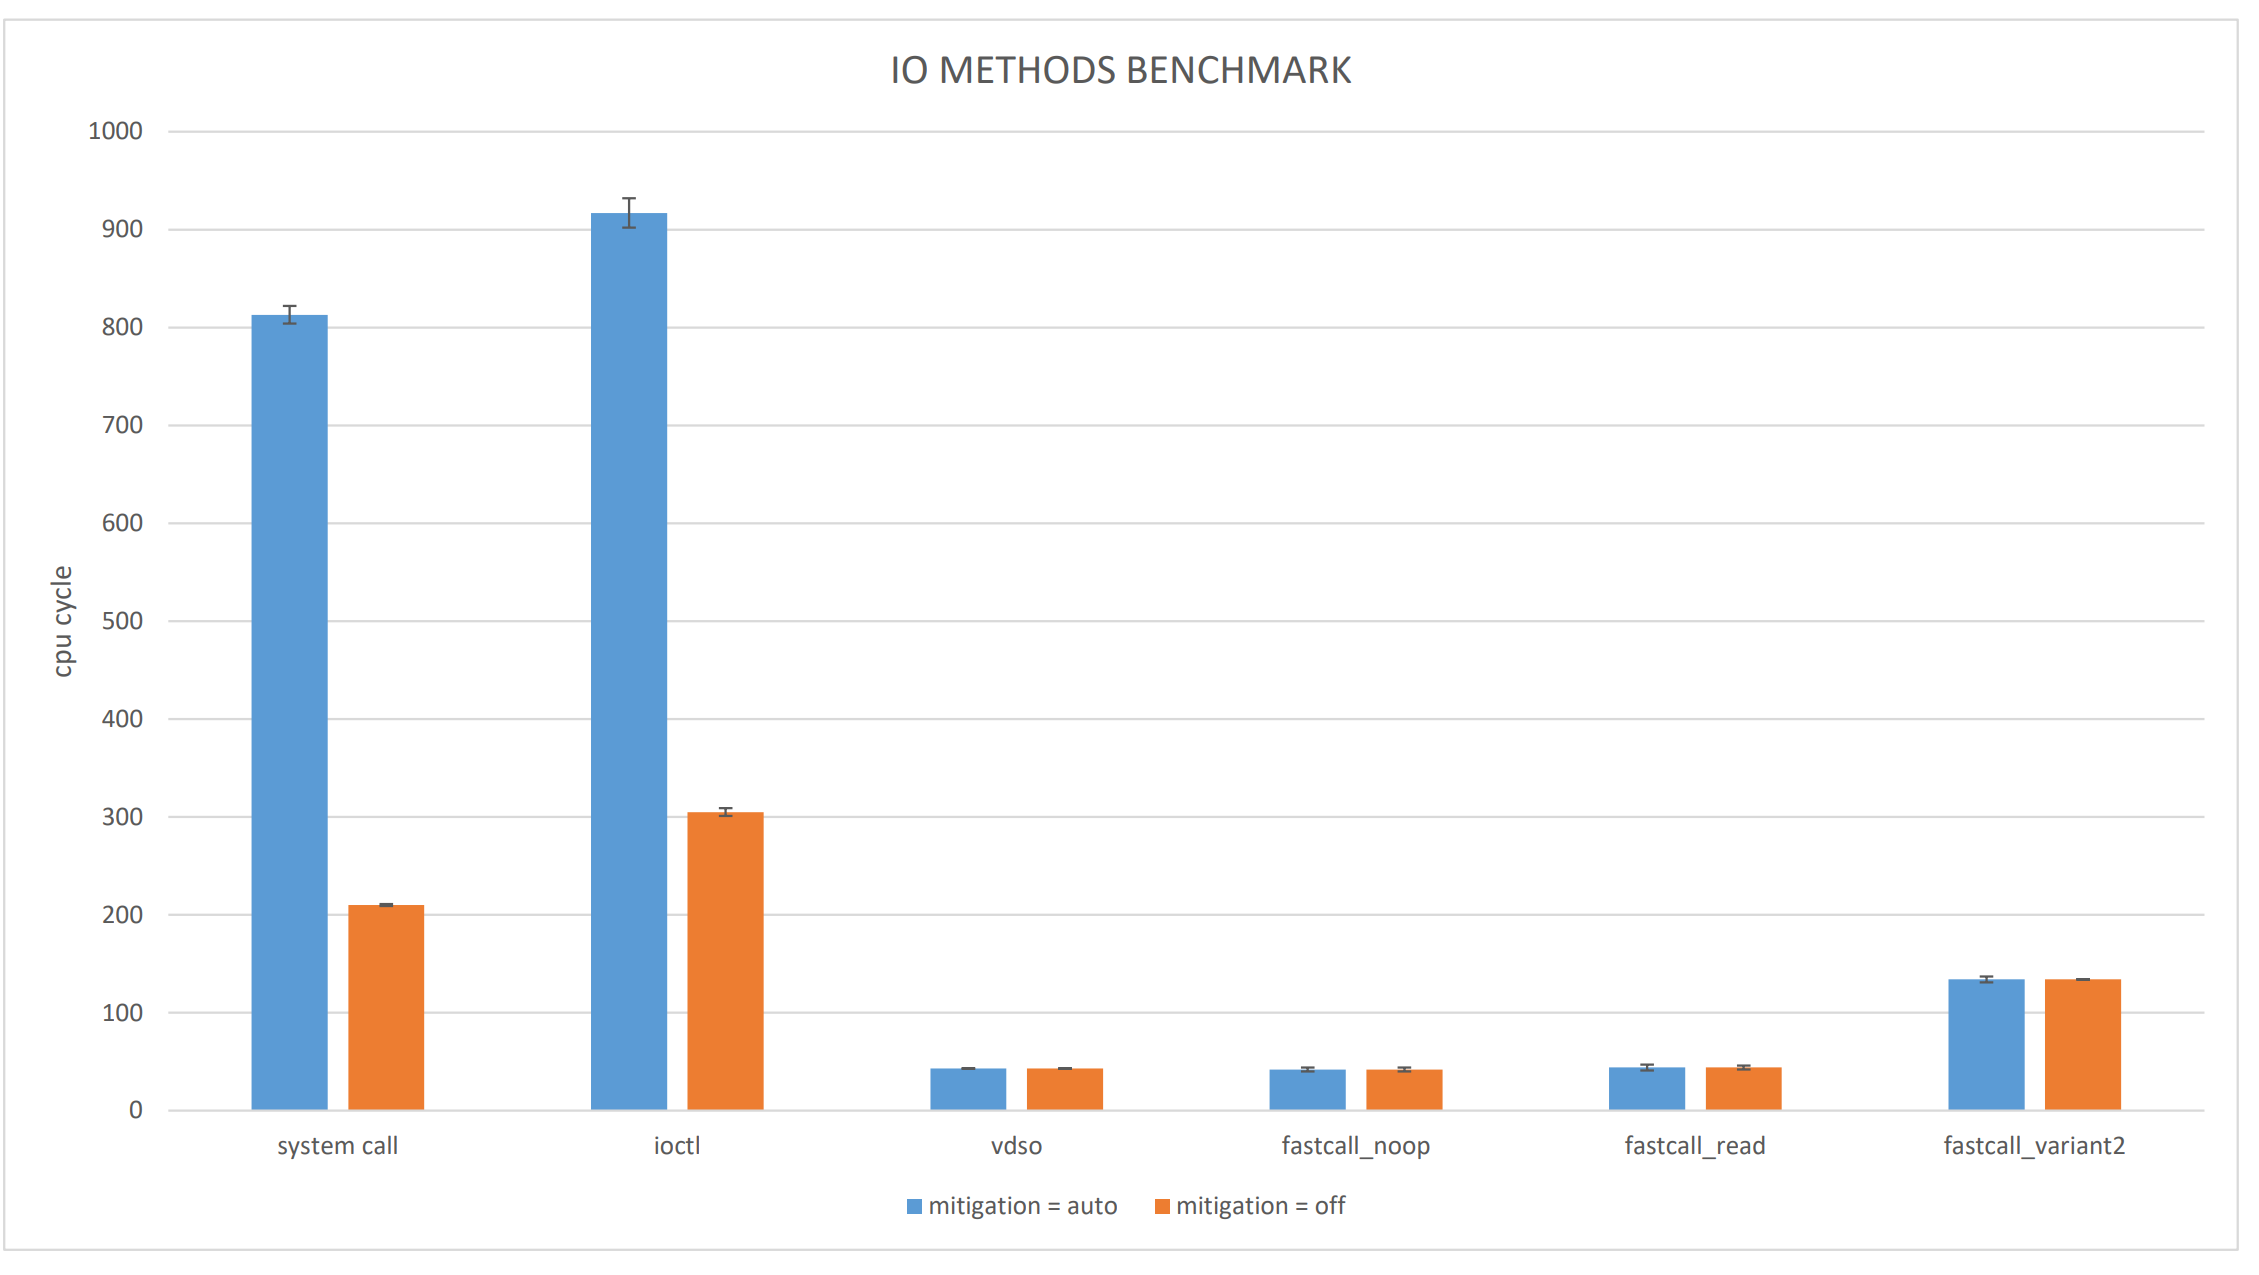
\includegraphics[width=0.8\textwidth]{images/IO_PERFORMANCE}
  \caption[IO performance benchmark]{IO performance benchmark}
   \label{fig:IO_PERFORMANCE}
\end{figure}

\begin{table}[htp]
  \centering
  \begin{tabular}{lrrr}
    \textbf{name} & \textbf{mean} & \textbf{median} & \textbf{std deviation} \\
    \hline
    \textit{system call empty} & 813 & 813 & 9\\
    \textit{ioctl empty} &917 & 916 & 15\\
    \textit{vdso empty} & 43 & 44 & 0\\
    \textit{fastcall empty} & 42 & 42 & 2\\
    \textit{fastcall read} & 44 & 44 & 3\\
    \textit{fastcall variant2 empty} & 134 & 135 & 3\\
    % \hline
    % \textit{total} & 88,215 & \unit[100]{\%} & \unit[23]{\%}\\

  \end{tabular}
  \caption[IO performance benchmark, mitigation = auto]{IO performance benchmark, mitigation = auto, unit: cpu cycle}
  \label{tab:numbers}
\end{table}

\begin{table}[htp]
  \centering
  \begin{tabular}{lrrr}
    \textbf{name} & \textbf{mean} & \textbf{median} & \textbf{std deviation} \\
    \hline
    \textit{system call empty} & 210 & 210 & 1\\
    \textit{ioctl empty} &305 & 305 & 4\\
    \textit{vdso empty} & 43 & 44 & 0\\
    \textit{fastcall empty} & 42 & 42 & 2\\
    \textit{fastcall read} & 44 & 44 & 2\\
    \textit{fastcall variant2 empty} & 134 & 135 & 0\\
    % \hline
    % \textit{total} & 88,215 & \unit[100]{\%} & \unit[23]{\%}\\

  \end{tabular}
  \caption[IO performance benchmark, mitigation = off]{IO performance benchmark, mitigation = off, unit: cpu cycle}
  \label{tab:number1}
\end{table}


First, let us view the performance comparison of different IO methods, i.e., 
system call empty function, ioctl empty function, vDSO empty function, fast call empty function, 
fast call read function, and fast call variant2 empty functionq. 
Note that the fast call read function is a fast call function that gets a secret 
from the secret region and reads one byte from the hidden region using the secret 
as the address. The fast call variant2 empty function represents an empty fast call 
function created by another fast call mechanism. The difference between the fast 
call empty function and the fast call variant2 empty function is that later one goes 
through the kernel.  Figure \ref{fig:IO_PERFORMANCE} shows the mean and standard deviation of different 
IO methods execution. Note that detailed data are listed in Tables ~\ref{tab:numbers} and ~\ref{tab:number1} 



It is not difficult to see from the figure that when the mitigation is 
turned on, the running speed of the fast call empty function is 20 times 
that of the system call and ioctl. This is expected because, in this case, 
context switching and page table switching are required when the system call 
and ioctl cross the user-kernel boundary.  On the other hand, compared with ioctl, 
the fast call read function can read the value of the device register mapped to the 
hidden region with only 44 CPU cycles. This undoubtedly dramatically improves the 
performance of IO. In particular, from comparing the fast call empty function 
and fast call variant two empty function, we can find that the fast call empty 
function is more than three times faster than the latter. Because the fast call 
variant two must suffer the performance penalty caused by the context switch 
in privilege transition. In addition, we found that the fast call function has 
no performance loss due to the mitigation since it is running totally on the 
user space. Correspondingly, when mitigation is turned on, the system call 
and ioctl suffer a significant performance loss because the page table needs 
to be switched additionally during the privilege transition. This has led 
to cache missed etc.



\begin{figure}[H]
  \centering
  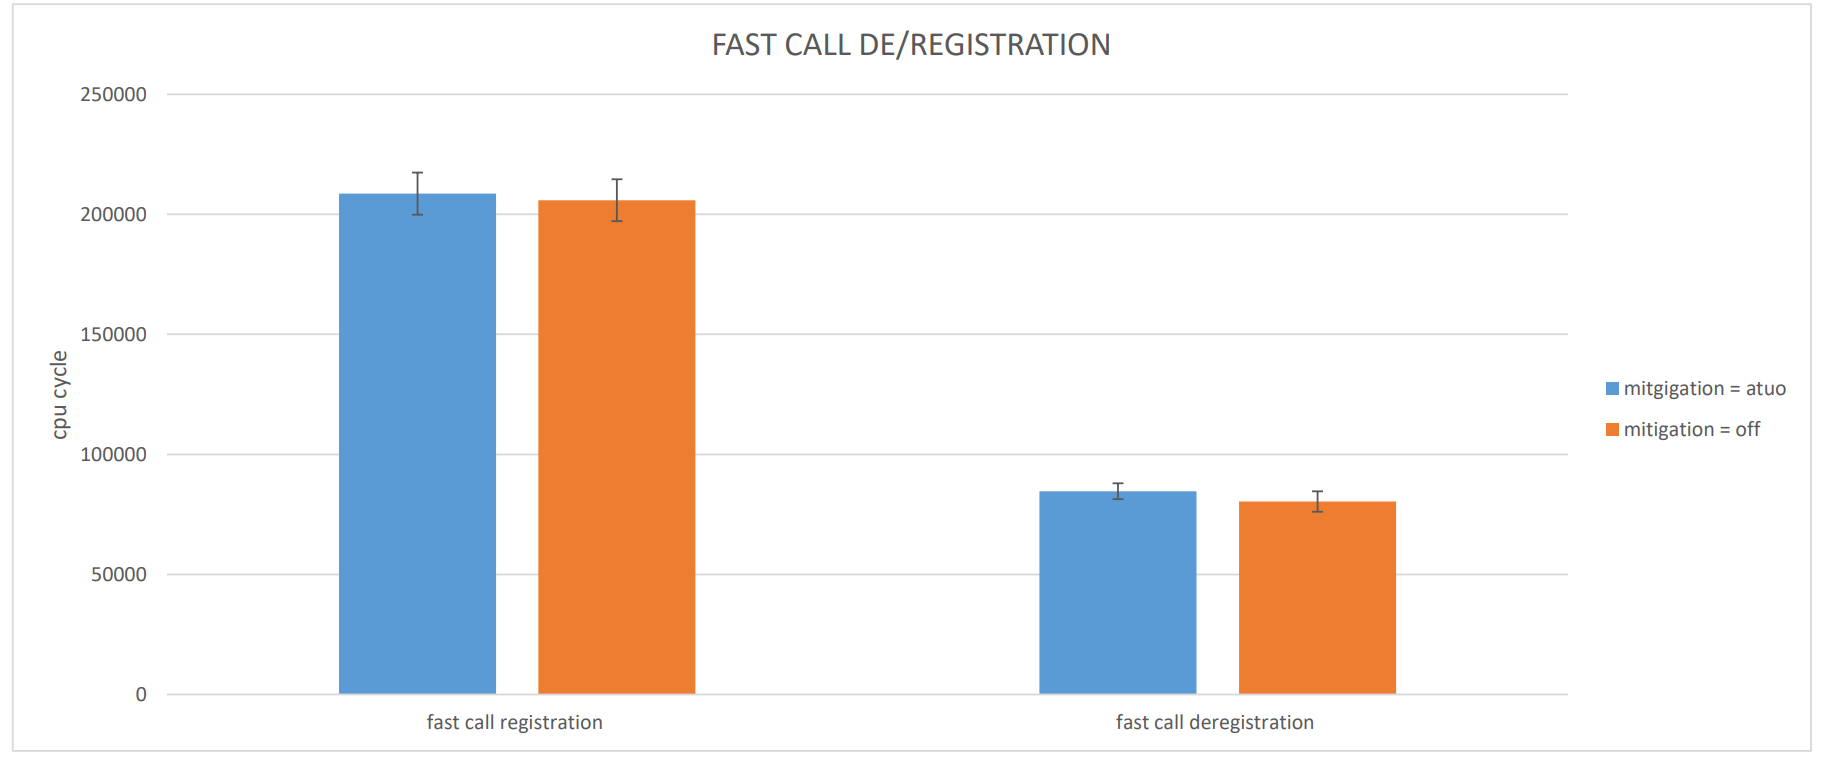
\includegraphics[width=0.8\textwidth]{images/rederegistration}
  \caption[Fast call de/registration benchmark]{Fast call de/registration benchmark}
   \label{fig:rederegistration}
\end{figure}

\begin{table}[htp]
  \centering
  \begin{tabular}{lrrr}
    \textbf{name} & \textbf{mean} & \textbf{median} & \textbf{std deviation} \\
    \hline
    \textit{fast call registration with mitigation} & 208643 & 210051 & 8776\\
    \textit{fast call registration without mitigation} & 205899 & 206473 & 8715\\


    
    % \hline
    % \textit{total} & 88,215 & \unit[100]{\%} & \unit[23]{\%}\\

  \end{tabular}
  \caption[Fast call registration benchmark]{Fast call registration benchmark, unit: cpu cycle}
  \label{tab:number2}
\end{table}


\begin{table}[htp]
  \centering
  \begin{tabular}{lrrr}
    \textbf{name} & \textbf{mean} & \textbf{median} & \textbf{std deviation} \\
    \hline
    \textit{fast call deregistration with mitigation} &84671 & 85097 & 3305\\
    \textit{fast call deregistration without mitigation} &80369 & 80542 & 4260\\
    % \hline
    % \textit{total} & 88,215 & \unit[100]{\%} & \unit[23]{\%}\\

  \end{tabular}
  \caption[Fast call deregistration benchmark]{Fast call deregistration benchmark, unit: cpu cycle}
  \label{tab:number3}
\end{table}


Figure \ref{fig:rederegistration} shows the time required to register a fast call 
and unregister a fast call. Because fast call registration 
and cancellation consume a lot of time, the mitigation's impact 
can be ignored. For detailed data, please refer to Tables ~\ref{tab:number2} and ~\ref{tab:number3}. 
There are many reasons why the fast call registration process is much 
slower than the fast call deregistration process. One of the essential 
reasons is that the fast mechanism dynamically allocates and initializes the fast call table 
when registering a fast call. In addition, during the fast call registration, 
the kernel's fast call infrastructure needs to traverse the fast call table 
multiple times, which also causes a considerable performance loss.


\begin{figure}[H]
  \centering
  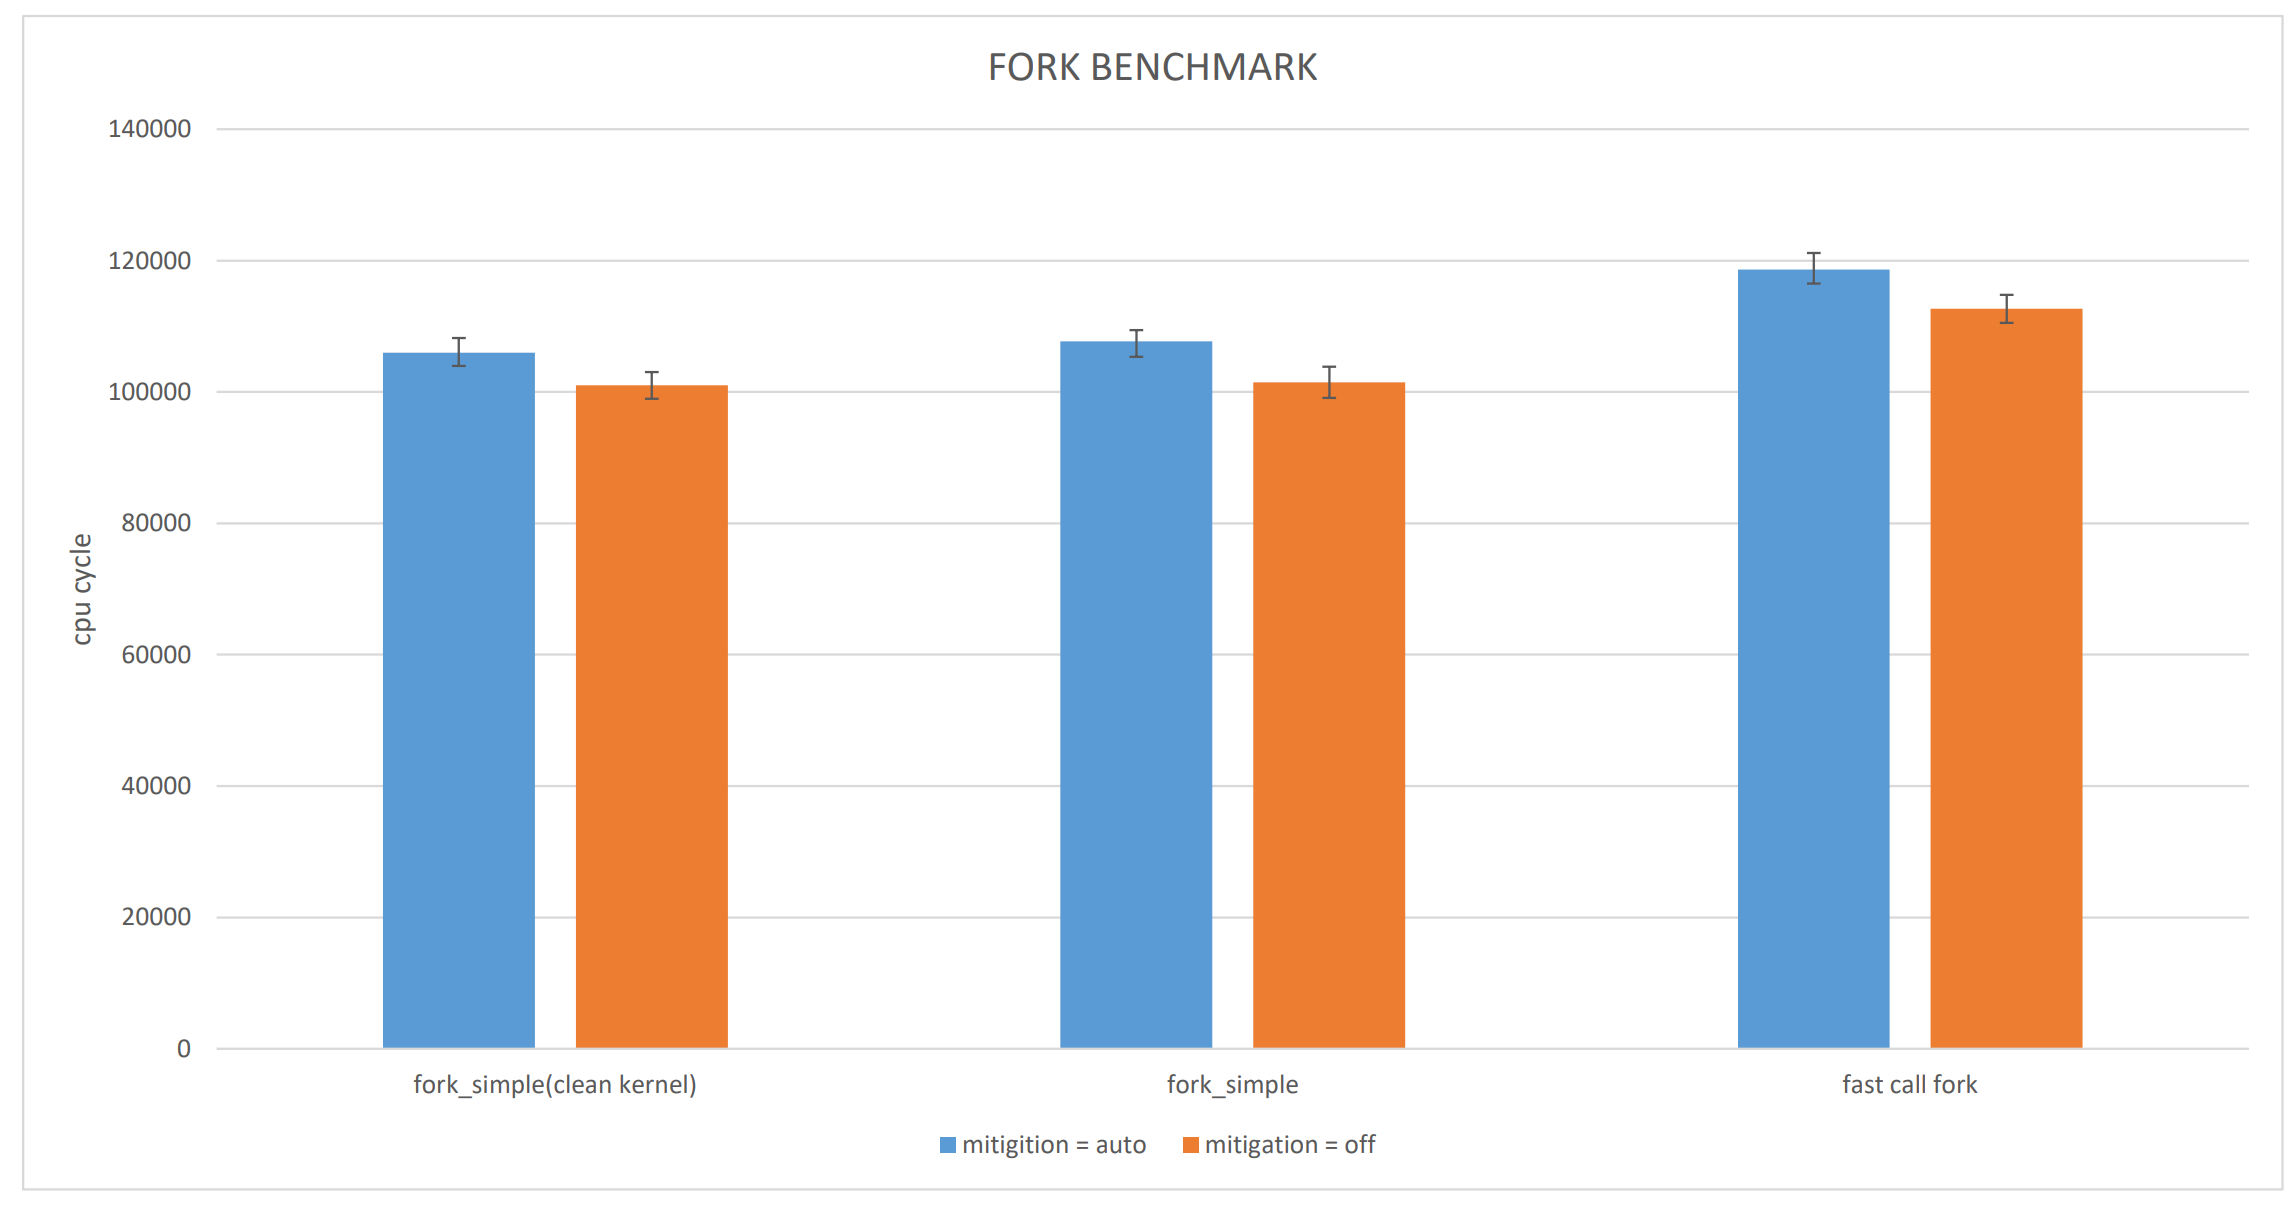
\includegraphics[width=0.8\textwidth]{images/FORK}
  \caption[FORK benchmark]{FORK benchmark}
   \label{fig:FORK}
\end{figure}


\begin{table}[htp]
  \centering
  \begin{tabular}{lrrr}
    \textbf{name} & \textbf{mean} & \textbf{median} & \textbf{std deviation} \\
    \hline
    \textit{fork simple(clean kernel)} & 105999 & 105546 & 2220\\
    \textit{fork simple} &107727 & 107398 & 1695\\
    \textit{fast call fork} & 118639 & 118144 & 2524\\
    % \hline
    % \textit{total} & 88,215 & \unit[100]{\%} & \unit[23]{\%}\\

  \end{tabular}
  \caption[FORK benchmark, mitigation = auto]{FORK benchmark, mitigation = auto, unit: cpu cycle}
  \label{tab:numbers4}
\end{table}


\begin{table}[htp]
  \centering
  \begin{tabular}{lrrr}
    \textbf{name} & \textbf{mean} & \textbf{median} & \textbf{std deviation} \\
    \hline
    \textit{fork simple(clean kernel)} & 100997 & 101011 & 2032\\
    \textit{fork simple} &101472 & 101009 & 2375\\
    \textit{fast call fork} & 112654 & 112216 & 2133\\
    % \hline
    % \textit{total} & 88,215 & \unit[100]{\%} & \unit[23]{\%}\\

  \end{tabular}
  \caption[FORK benchmark, mitigation = off]{FORK benchmark, mitigation = off, unit: cpu cycle}
  \label{tab:numbers5}
\end{table}

As shown in the figure, we first tested the running speed of a 
regular fork operation(fork simple) on the kernel  
and without fast call implementation. Subsequently, we tested the 
average execution speed of the fork(fast call fork) when the parent process registered 
50 fast calls, and each fast call had 6 VMAs\emph{10.5555/983550}. It can be seen from the 
figure that the regular fork operation runs at the same speed no matter 
the kernel has the fast call implementation. 
Interestingly, the average running time of \emph{fast call fork} is 10,000 cycles 
longer than that of the \emph{simple fork}. This reason is that the parent process 
in the \emph{fast call fork} has 50*6 VMAs more than the parent process in the \emph{simple fork}. 
Although the VMAs belonging to the fast call cannot be copied during the 
fork process, the kernel still needs to traverse these 300 VMAs and call 
functions to modify the metadata about VMAs in the virtual address 
space descriptor\emph{10.5555/983550} and other places.


\section{Meltdown attack mitigation}

CPU side-channel attacks\cite{3,4} severely impact our fast call 
mechanism since fast call's components run on the user space, 
i.e., without kernel protection. Specifically, a fast call keeps its secret 
in the secret region, and the secret region relies on the permission bit on 
the page table entry to avoid any malicious user from reading this region. 
Remember that we discussed in the implementation chapter that the x86 architecture does not 
support executable-only pages.  Here, even if the x86 architecture supports 
only executable pages in the future, i.e., add a new permission bit for 
executable-only on \emph{PTE}\cite{25},  we cannot prevent attackers from using meltdown to 
attack this area. Now let us review the code snippet in the chapter \ref{sec:state} and see how an attacker uses this code to steal the secret(64-bit) in the 
secret region. Here we assume that the x86 architecture already supports 
executable-only pages.

\begin{lstlisting}[style=CStyle]
    char buf[8192]
  
    // the Flush of Flush+Reload
    clflush buf[0]
    clflush buf[4096]
  
    <some expensive instruction like divide>
  
    r1 = <a secret region virtual address>
    r2 = *r1
    r2 = r2 & 1      // speculated
    r2 = r2 * 4096   // speculated
    r3 = buf[r2]     // speculated
  
    <handle the page fault from "r2 = *r1">
  
    // the Reload of Flush+Reload
    a = rdtsc
    r0 = buf[0]
    b = rdtsc
    r1 = buf[4096]
    c = rdtsc
    if b-a < c-b:
      low bit was probably a 1
  \end{lstlisting}
  In this code snippet\cite{1}, the attacker first flushes the cache so that no 
  records related to \emph{buf[0]} and \emph{buf[4096]} exist in the cache. Then the 
  attacker lets the \emph{multi-core CPU} execute a costly instruction.  
  Instead of waiting for the completion of the instruction, the CPU 
  executes the following instructions speculatively. Remember, we discussed 
  in the chapter technical background that the CPU executes instructions 
  from lines 10 to 13 before checking whether the instructions are valid. 
  This means that the CPU checks the permission bit \emph{executable only} on  
  \emph{PTE} corresponding to the page mapped to the secret region after it 
  obtains the secret stored on the secret region and complete the 
  code in line 12 and 13.  In other words,  in line 10 of the above 
  code snippet,  the CPU first tries to load the secret from the 
  cache directly. If it is a load miss, the secret data is fetched 
  from memory to register \emph{r2,} and the CPU puts it into the cache. 
  Then the CPU executes the instructions in lines 11, 12, 13 and 
  puts the value of \emph{buf[0]} or \emph{buf[4096]} to the cache based on 
  the first bit of the secret.  Later, during the instruction 
  retirement stage, the CPU checks whether the instruction in 
  line 10 is valid based on the permission bit on \emph{PTE} and reverts 
  its state since the execution from lines 10 to 13 are not permitted. 
  However, everything is too late. The value of \emph{buf[0]} or \emph{buf[4096]} 
  is already cached, and the CPU cannot revert the cache state. 
  Therefore, the attacker can then guess the secret by cache timing\cite{11}. 
  In the end, the attacker can get the secret by executing this code 
  snippet 64 times, each time guessing 1 bit of the secret.

  On top of that, the same things happened if we also set \emph{cache disable bit} 
  on the secret page's \emph{PTE}.  In this case, any data 
  that is on the secret page will not be cached(the code in line 
  13 will not be cached).  This means,  in line 10 of the above code snippet, 
  after the secret is fetched from memory to register r2, the CPU won't 
  put it into the cache.  However, the meltdown attack does not rely on the 
  secret directly.  Instead, the attacker uses flush and reload to check 
  whether \emph{buf[0]} or \emph{buf[4096]} is in the cache. Therefore, it does not 
  matter whether the secret is in the cache.  In particular, there is no 
  way to avoid the buffer from being uncached since the attacker allocates 
  the buffer and does not set the \emph{cache-disable bit} on \emph{PTE}. Thus, we can't
   protect the secret region using the permission bit \emph{executable-only}
   and the cache-disable bit on \emph{PTE}.
  


   

  Because the meltdown attack is mainly composed of out-of-order 
  execution and covert channel, mitigation methods can start from 
  these two aspects. The second aspect would be more complicated 
  since there are multiple potential convert channels, including 
  cache, heat, etc.  So we decided to start from the first aspect. 
  Here our goal is to prevent the secret from being accessed by 
  unauthorized users. To achieve this goal, we argue that the CUP 
  must be redesigned.  More specifically, the CPU should execute 
  the memory-access related instruction(load data from memory or 
  store data to memory) in the following order\cite{3}:
  \begin{itemize}
    \item Before the speculative memory fetch operation, the CPU should first check the permission bits on PTE. 
    \item If the permission check is failed, zero should be returned instead of the real data.
  \end{itemize}
  In this way, the instructions in line 10 load zero into \emph{r2}. 
  Therefore, the attacker cannot guess the secret anymore. Particularly, the secret is not cached too since the CPU cache the secret after 
  it checks the permission bit. Note that AMD CPUs obviously work in
  this way all along, which means Meltdown does work on any of AMD CPUs\cite{26}.


\section{Spectre attack mitigation}

After changing the CPU behavior in out-of-order execution, 
attackers can no longer guess any data they do not have permission 
to access, i.e., privilege escalation. However, attackers can still 
exploit the \emph{Spectre vulnerability}\cite{4} to tamper devices through fast calls. 
Specifically, an attacker process can poison the branch predictor 
shared by all processes running on the same CPU so that the victim 
process that has registered fast calls would jump to a gadget chosen 
by the attacker. Since device registers are directly mapped onto the 
user space(hidden regions), the gadget may trick the victim into 
exploring the user space and finding the hidden regions. 
In order to deal with this situation, we divide the user space into two 
parts and assign the upper part of the user space to the hidden regions. 
In the upper part of the user space, any page fault kills the process 
directly, and processes are not allowed to allocate any memory, 
which means a malicious attacker cannot handle the page fault in 
some way and find the hidden region by exploring the user space anymore. 
In this case, while executing the code in the gadget, the victim only 
has one chance to guess the location of hidden regions. If the guess is 
wrong, the page fault handler sends \emph{SEGKILL}\cite{21} to the 
victim so that the 
victim has no choice but to kill itself. Therefore, we minimize the 
possibility of the hidden area being attacked successfully.

To further minimize the \emph{Spectre attack}, we need to put in more effort. 
Here, our goal is to prevent the victim jumps to the gadget based on the wrong 
records in the predictor.  One possible software solution is to design a tool 
that can limit the wrong speculations. For example, Google's Retpoline patch can 
detect and overwrite all dangerous branches that may affect \emph{Spectre Variant 2}. 
In this case, Google's Retpoline patch forces the CPU to jump to an empty gadget 
after it executes the branch speculatively\cite{5}. A more solid solution is introducing 
new instructions\cite{5}.  For example, the hardware engineer could add new instructions 
that allow the operating system to empty the predictor in certain situations. 
An ultimate solution would be redesigning the CPU architecture. The CPU architecture 
should have dedicated hardware for speculative execution that is separated from other 
CPU structures, especially the cache. Any speculatively executed operations should be 
invisible before those operations are committed\cite{5}.  
 \cleardoublepage

%%% Local Variables:
%%% TeX-master: "diplom"
%%% End:
